\documentclass{Configuration_Files/PoliMi3i_thesis}

%------------------------------------------------------------------------------
%	REQUIRED PACKAGES AND  CONFIGURATIONS
%------------------------------------------------------------------------------

% CONFIGURATIONS
\usepackage{parskip} % For paragraph layout
\usepackage{setspace} % For using single or double spacing
\usepackage{emptypage} % To insert empty pages
\usepackage{multicol} % To write in multiple columns (executive summary)
\setlength\columnsep{15pt} % Column separation in executive summary
\setlength\parindent{0pt} % Indentation
\raggedbottom  

% PACKAGES FOR TITLES
\usepackage{titlesec}
% \titlespacing{\section}{left spacing}{before spacing}{after spacing}
\titlespacing{\section}{0pt}{3.3ex}{2ex}
\titlespacing{\subsection}{0pt}{3.3ex}{1.65ex}
\titlespacing{\subsubsection}{0pt}{3.3ex}{1ex}
\usepackage{color}

% PACKAGES FOR LANGUAGE AND FONT
\usepackage[utf8]{inputenc} % UTF8 encoding
\usepackage[T1]{fontenc} % Font encoding
\usepackage[11pt]{moresize} % Big fonts
\usepackage{pythonhighlight}

% PACKAGES FOR IMAGES
\usepackage{graphicx}
\usepackage{transparent} % Enables transparent images
\usepackage{eso-pic} % For the background picture on the title page
\usepackage{subfig} % Numbered and caption subfigures using \subfloat.
\usepackage{tikz} % A package for high-quality hand-made figures.
\usetikzlibrary{}
\graphicspath{{./Images/}} % Directory of the images
\usepackage{caption} % Coloured captions
\usepackage{xcolor} % Coloured captions
\usepackage{amsthm,thmtools,xcolor} % Coloured "Theorem"
\usepackage{float}

% STANDARD MATH PACKAGES
\usepackage{amsmath}
\usepackage{amsthm}
\usepackage{amssymb}
\usepackage{amsfonts}
\usepackage{bm}
\usepackage[overload]{empheq} % For braced-style systems of equations.
\usepackage{fix-cm} % To override original LaTeX restrictions on sizes

% PACKAGES FOR TABLES
\usepackage{tabularx}
\usepackage{longtable} % Tables that can span several pages
\usepackage{colortbl}

% PACKAGES FOR ALGORITHMS (PSEUDO-CODE)
\usepackage{algorithm}
\usepackage{algorithmic}

% PACKAGES FOR REFERENCES & BIBLIOGRAPHY
\usepackage[colorlinks=true,linkcolor=black,anchorcolor=black,citecolor=black,filecolor=black,menucolor=black,runcolor=black,urlcolor=black]{hyperref} % Adds clickable links at references
\usepackage{cleveref}
\usepackage[square, numbers, sort&compress]{natbib} % Square brackets, citing references with numbers, citations sorted by appearance in the text and compressed
\bibliographystyle{abbrvnat} % You may use a different style adapted to your field

% OTHER PACKAGES
\usepackage{pdfpages} % To include a pdf file
\usepackage{afterpage}
\usepackage{lipsum} % DUMMY PACKAGE
\usepackage{fancyhdr} % For the headers
\fancyhf{}

% Input of configuration file. Do not change config.tex file unless you really know what you are doing. 
% Define blue color typical of polimi
\definecolor{bluepoli}{cmyk}{0.4,0.1,0,0.4}

% Custom theorem environments
\declaretheoremstyle[
  headfont=\color{bluepoli}\normalfont\bfseries,
  bodyfont=\color{black}\normalfont\itshape,
]{colored}

% Set-up caption colors
\captionsetup[figure]{labelfont={color=bluepoli}} % Set colour of the captions
\captionsetup[table]{labelfont={color=bluepoli}} % Set colour of the captions
\captionsetup[algorithm]{labelfont={color=bluepoli}} % Set colour of the captions

\theoremstyle{colored}
\newtheorem{theorem}{Theorem}[chapter]
\newtheorem{proposition}{Proposition}[chapter]

% Enhances the features of the standard "table" and "tabular" environments.
\newcommand\T{\rule{0pt}{2.6ex}}
\newcommand\B{\rule[-1.2ex]{0pt}{0pt}}

% Pseudo-code algorithm descriptions.
\newcounter{algsubstate}
\renewcommand{\thealgsubstate}{\alph{algsubstate}}
\newenvironment{algsubstates}
  {\setcounter{algsubstate}{0}%
   \renewcommand{\STATE}{%
     \stepcounter{algsubstate}%
     \Statex {\small\thealgsubstate:}\space}}
  {}

% New font size
\newcommand\numfontsize{\@setfontsize\Huge{200}{60}}

% Title format: chapter
\titleformat{\chapter}[hang]{
\fontsize{50}{20}\selectfont\bfseries\filright}{\textcolor{bluepoli} \thechapter\hsp\hspace{2mm}\textcolor{bluepoli}{|   }\hsp}{0pt}{\huge\bfseries \textcolor{bluepoli}
}

% Title format: section
\titleformat{\section}
{\color{bluepoli}\normalfont\Large\bfseries}
{\color{bluepoli}\thesection.}{1em}{}

% Title format: subsection
\titleformat{\subsection}
{\color{bluepoli}\normalfont\large\bfseries}
{\color{bluepoli}\thesubsection.}{1em}{}

% Title format: subsubsection
\titleformat{\subsubsection}
{\color{bluepoli}\normalfont\large\bfseries}
{\color{bluepoli}\thesubsubsection.}{1em}{}

% Shortening for setting no horizontal-spacing
\newcommand{\hsp}{\hspace{0pt}}

\makeatletter
% Renewcommand: cleardoublepage including the background pic
\renewcommand*\cleardoublepage{%
  \clearpage\if@twoside\ifodd\c@page\else
  \null
  \AddToShipoutPicture*{\BackgroundPic}
  \thispagestyle{empty}%
  \newpage
  \if@twocolumn\hbox{}\newpage\fi\fi\fi}
\makeatother

%For correctly numbering algorithms
\numberwithin{algorithm}{chapter}

%----------------------------------------------------------------------------
%	NEW COMMANDS DEFINED
%----------------------------------------------------------------------------

% EXAMPLES OF NEW COMMANDS
\newcommand{\bea}{\begin{eqnarray}} % Shortcut for equation arrays
\newcommand{\eea}{\end{eqnarray}}
\newcommand{\e}[1]{\times 10^{#1}}  % Powers of 10 notation

%----------------------------------------------------------------------------
%	ADD YOUR PACKAGES (be careful of package interaction)
%----------------------------------------------------------------------------
\definecolor{codegreen}{rgb}{0,0.6,0}
\definecolor{codegray}{rgb}{0.5,0.5,0.5}
\definecolor{codepurple}{rgb}{0.58,0,0.82}
\definecolor{backcolour}{rgb}{0.95,0.95,0.92}
\usepackage{color}   %May be necessary if you want to color links
\usepackage{hyperref}
\usepackage{graphicx}
\usepackage[utf8]{inputenc}
\usepackage{listings}
\usepackage{xcolor}
\hypersetup{
colorlinks=true, %set true if you want colored links
linktoc=all,     %set to all if you want both sections and subsections linked
linkcolor=black,  %choose some color if you want links to stand out
urlcolor=blue,
}
\lstdefinestyle{mystyle}{
backgroundcolor=\color{backcolour},
commentstyle=\color{codegreen},
keywordstyle=\color{magenta},
numberstyle=\tiny\color{codegray},
stringstyle=\color{codepurple},
basicstyle=\ttfamily\footnotesize,
breakatwhitespace=false,
breaklines=true,
captionpos=b,
keepspaces=true,
numbers=left,
numbersep=5pt,
showspaces=false,
showstringspaces=false,
showtabs=false,
tabsize=2
}

\lstset{style=mystyle}


%----------------------------------------------------------------------------
%	ADD YOUR DEFINITIONS AND COMMANDS (be careful of existing commands)
%----------------------------------------------------------------------------

%----------------------------------------------------------------------------
%	BEGIN OF YOUR DOCUMENT
%----------------------------------------------------------------------------

\begin{document}

\fancypagestyle{plain}{%
\fancyhf{} % Clear all header and footer fields
\fancyhead[RO,RE]{\thepage} %RO=right odd, RE=right even
\renewcommand{\headrulewidth}{0pt}
\renewcommand{\footrulewidth}{0pt}}

%----------------------------------------------------------------------------
%	TITLE PAGE
%----------------------------------------------------------------------------

\pagestyle{empty} % No page numbers
\frontmatter % Use roman page numbering style (i, ii, iii, iv...) for the preamble pages

\puttitle{
title=SMBUD Project - Spark,
name1=Gabriele Ginestroni, % Author Name and Surname
name2=Giacomo Gumiero,
name3=Lorenzo Iovine,
name4=Nicola Landini,
name5=Francesco Leone,
academicyear=2022-2023,
groupnumber=10
} % These info will be put into your Title page


%----------------------------------------------------------------------------
%	PREAMBLE PAGES: ABSTRACT (inglese e italiano), EXECUTIVE SUMMARY
%----------------------------------------------------------------------------
\startpreamble
\setcounter{page}{1} % Set page counter to 1

%----------------------------------------------------------------------------
%	LIST OF CONTENTS/FIGURES/TABLES/SYMBOLS
%----------------------------------------------------------------------------

% TABLE OF CONTENTS
\thispagestyle{empty}
\tableofcontents % Table of contents 
\thispagestyle{empty}
\cleardoublepage

%-------------------------------------------------------------------------
%	THESIS MAIN TEXT
%-------------------------------------------------------------------------
% In the main text of your thesis you can write the chapters in two different ways:
%
%(1) As presented in this template you can write:
%    \chapter{Title of the chapter}
%    *body of the chapter*
%
%(2) You can write your chapter in a separated .tex file and then include it in the main file with the following command:
%    \chapter{Title of the chapter}
%    \input{chapter_file.tex}
%
% Especially for long thesis, we recommend you the second option.

\addtocontents{toc}{\vspace{2em}} % Add a gap in the Contents, for aesthetics
\mainmatter % Begin numeric (1,2,3...) page numbering

\chapter{Introduction}
\label{ch:introduction}
In this chapter will be presented the problem specification and the hypothesis under which the database is implemented.

\section{Problem Specification}
This project aims to build a database that handles scientific articles contained in the DBLP bibliography. In this implementation,
our work will be focused on \emph{Spark} technology, which is a ditributed computing infrastructure that can process large amount of data in efficient day. To accomplish this we used the PySpark interface that allows us to interact with Apache Spark using python. 

\section{Assumption}
\begin{itemize}
    \item An author can't work for more than one organization for the same Publication
    \item As in the MongoDB implementation, a publication can be published only in one venue
    \item Venues with the same raw take place in the same city
    \item Venue is identified by raw field
\end{itemize}

\chapter{Conceptual Model}
\label{ch:conc_model}
\begin{figure}[H]
\centering
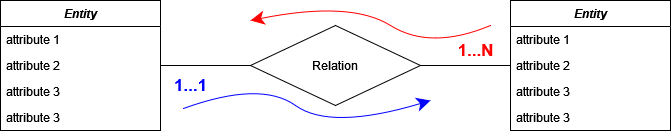
\includegraphics[width=0.6\textwidth]{legendaER.png}
\caption{ER Diagram Organization}
\label{fig:erleg}
\end{figure}
\begin{figure}[H]
\centering
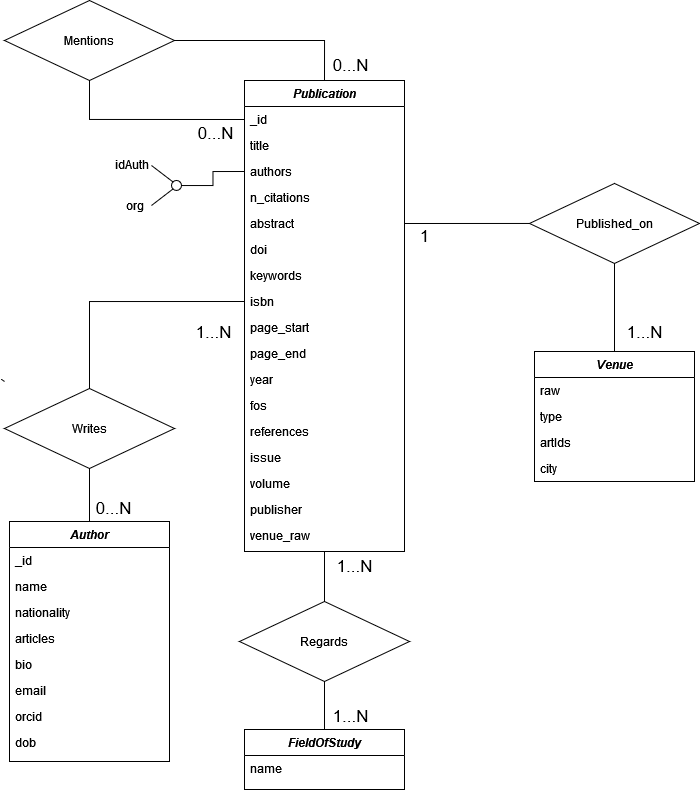
\includegraphics[width=0.75\textwidth]{ERSpark.png}
\caption{Conceptual Model}
\label{fig:er}
\end{figure}

\textbf{Note:} in the conceptual model diagram, we highlighted the primary keys of the entities that are implemented as a collection:
\emph{Publication}, \emph{Author} and \emph{Venue}

The conceptual model above contains 4 main entities:
\begin{itemize}
    \item \textbf{Publication:} represents all the scientific articles. Its attributes are: \emph{\_id, title, n\_citations,
        abstract, doi, keywords, isbn, page\_start, page\_end, year, fos} and its
        organization will be presented later
    \item \textbf{Author:} it is the one who contributed to a publication. Its attributes are: \emph{\_id, name, nationality,
        bio, email, orcid, dob (date of birth)}
    \item \textbf{Venue:} it is where a publication is published or presented. Its attributes are: \emph{raw, type,
        city}
    \item \textbf{FieldOfStudy:} this entity represents the subjects of the publication and its attribute is \emph{name}
\end{itemize}

\bigskip
The 4 main entities just described, are related to each other through the following relationships:
\begin{itemize}
    \item \textbf{References:} is the relationship between a \emph{publication} and another \emph{publication} cited by the first one
    \item \textbf{Published\_on:} is the relationship between a \emph{publication} and its \emph{venue}. Its attributes are: \emph{ issue, volume, publisher}
    \item \textbf{Writes:} is the relationship between \emph{author} and \emph{publication} which features the affiliation property.
        We decided to design it with \verb |org| as an attribute of the relationship, due to the fact that it belongs
        only to a pair of \emph{author} and \emph{publication} and it represents the institute where the author worked for the publication
    \item \textbf{Regards:} is the relationship between a \emph{publication} and its \emph{fields of study}
\end{itemize}

\bigskip
Differences with \emph{MongoDB} conceptual model:
\begin{itemize}
\item we add field \verb |city| in \emph{Venue} entity representing the location of the venue
\item \emph{Chapters} and \emph{images} have been removed
\end{itemize}


\chapter{Data Structure}
\label{ch:data_struct}
In this part of the project we used the same two \verb|JSON|s used in the \emph{MongoDB} implementation. We only removed
chapters inside articles and \verb|_id| authors inside articles was renamed as \verb|idAuth|. Also id and dates were reconverted
in plain text because in \emph{MongoDB} we needed to add them as special entities: \verb|$oid| and \verb|$date|.\newline
This was done via the following lines of script:
\begin{itemize}
    \item the \textbf{first line} is used for the \verb |JSON| file containing the articles. The script removes \verb|$oid|, to
        delete chapters field and to rename authors field \emph{id} into \emph{idAuth}
    \item the \textbf{second line} is used for the \verb |JSON| file containing the authors. The script removes \verb|$oid| and
        \verb|$date| \\
\end{itemize}
\begin{lstlisting}
cat dblp_sample_filtered.json | sed -E 's/\{"\$oid":(["a-z0-9]+)\}/\1/g' | jq 'del(.[].chapters)' | jq '.[].authors[] |= with_entries(if .key == "id" then .key = "idAuth" else . end)' > dblp_sample_filtered_spark.json

cat dblp_sample_reverted_filtered.json | sed -E 's/\{"\$oid":(["a-z0-9]+)\}/\1/g' | sed -E 's/\{"\$date":(["A-Z0-9:-]+)\}/\1/g' > dblp_sample_reverted_filtered_spark.json
\end{lstlisting}

\chapter{Dataframe Structure}
\label{ch:frame_struct}
\section{Article Structure}
\begin{lstlisting}
root
|-- _id: string (nullable = true)
|-- title: string (nullable = true)
|-- authors: array (nullable = true)
|    |-- element: struct (containsNull = true)
|    |    |-- idAuth: string (nullable = true)
|    |    |-- org: string (nullable = true)
|-- n_citation: integer (nullable = true)
|-- abstract: string (nullable = true)
|-- doi: string (nullable = true)
|-- keywords: array (nullable = true)
|    |-- element: string (containsNull = true)
|-- isbn: string (nullable = true)
|-- page_start: string (nullable = true)
|-- page_end: string (nullable = true)
|-- year: integer (nullable = true)
|-- fos: array (nullable = true)
|    |-- element: string (containsNull = true)
|-- references: array (nullable = true)
|    |-- element: string (containsNull = true)
|-- issue: string (nullable = true)
|-- volume: string (nullable = true)
|-- publisher: string (nullable = true)
|-- venue_raw: string (nullable = true)
\end{lstlisting}
The structure just shown represents an \emph{Article}; its attributes are:
\begin{itemize}
    \item \textbf{\_id} is the identifier of a publication.
    \item \textbf{title} represents the title of the publication.
    \item \textbf{authors} is an array that contains: \verb |idAuth| of the authors of the article and the \verb |org|
        field which represent the affiliation.
    \item \textbf{n\_citation} is the number of times that the publication has been mentioned.
    \item \textbf{abstract} is a string containing a brief summary of the contents of the paper.
    \item \textbf{doi} Digital Object Identifier is a persistent and standardized identifier.
    \item \textbf{keywords} is an array containing keywords of the publication.
    \item \textbf{isbn} is an identification code of the venue of the publication.
    \item \textbf{page\_start} defines the starting page of the publication.
    \item \textbf{page\_end} defines the last page of the publication.
    \item \textbf{year} represents the year of publication.
    \item \textbf{fos} is an array containing the fields of study of the publication.
    \item \textbf{references} set of ObjectIds of the referenced articles.
    \item \textbf{issue} refers to how many times a periodical has been published during that year.
    \item \textbf{volume} is the volume of the venue in which the article has been published.
    \item \textbf{publisher} is the name of the publisher of the article.
    \item \textbf{venue\_raw} is the name or the abbreviation of the venue (regardless the year, issue or volume) in which the
        publication was presented.
\end{itemize}
We moved \verb|issue|, \verb|volume| and \verb|publisher| to the \emph{Publication} structure because in this implementation we have a new 		       collection for the \emph{Venue}. This has been done because, as in previous projects, we decided to aggregate the venues with respect to the field \verb|raw|.

\section{Author Structure}
\begin{lstlisting}
root
|-- _id: string (nullable = true)
|-- name: string (nullable = true)
|-- nationality: string (nullable = true)
|-- articles: array (nullable = true)
|    |-- element: string (containsNull = true)
|-- bio: string (nullable = true)
|-- email: string (nullable = true)
|-- orcid: string (nullable = true)
|-- dob: timestamp (nullable = true)
\end{lstlisting}
The structure just shown represents an \emph{Author}; its attributes are:
\begin{itemize}
    \item \textbf{\_id} is the identifier of an author.
    \item \textbf{name} is the name of the author.
    \item \textbf{nationality} is the nationality of the author.
    \item \textbf{articles} is a set of articles identifier of the publications of the author.
    \item \textbf{bio} is a string that describes the author.
    \item \textbf{email} is the email address of the author.
    \item \textbf{orcid} Open Researcher and Contributor ID is a unique identifier for authors of scientific articles.
    \item \textbf{dob} is the birth date of the author.
\end{itemize}

\section{Venue Structure}
\begin{lstlisting}
root
|-- raw: string (nullable = true)
|-- type: integer (nullable = true)
|-- artIds: array (nullable = false)
|    |-- element: string (containsNull = false)
|-- city: string (nullable = true)
\end{lstlisting}
The structure just shown represents a \emph{Venue}. This dataframe was obtained extracting venues fields from the Articles dataframe already imported. \emph{Venue} attribute are the following:
\begin{itemize}
    \item \textbf{raw} is the name or the abbreviation of the venue (regardless the year, issue or volume) in which the
        publication was presented.
    \item \textbf{type} indicates the type of the publication.
    \item \textbf{artIds} is a set of articles identifier associated to the venue.
    \item \textbf{city} represents the location of the venue an it is randomly populated.
\end{itemize}
Note that \emph{artIds, city} where not present in the Article dataframe so have been generated during the creation of the venue collection. 

\newpage
\section{Dataframe Analysis}
These are the number of rows in our dataframes
\begin{figure}[H]
\centering
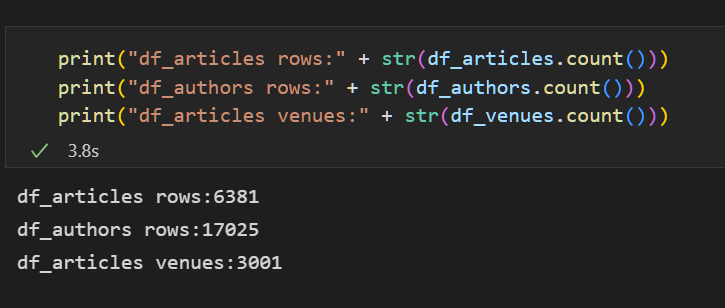
\includegraphics[width=0.8\textwidth]{dataframe_rows.PNG}
\label{fig:dataframe_dim}
\end{figure}



\chapter{Commands and Queries}
\label{ch:ceq}
\section{Commands}
We have identified the following \verb |INSERT| and \verb |UPDATE| commands to show the system basic functionalities.

\subsection{Insert a new author}
\label{auth_insert}
Assuming it is not present in the dataset, we created a row for the new author and we added into to the \emph{Author}'s dataframe.\newline
\begin{python}
new_author = Row(
    _id="638db170ae9ea0d19fad7a79",
    name="Emanuele Delle Valle ",
    nationality="it",
    articles=[],
    bio="Emanuele Della Valle holds a PhD in Computer Science from the \
        Vrije Universiteit Amsterdam and a Master degree in Computer Science\
        and Engineering from Politecnico di Milano. He is associate professor\
        at the Department of Electronics, Information and Bioengineering of\
        the Politecnico di Milano.",
    email="emanuele.dellavalle@gmail.com ",
    orcid="0000-0002-5176 -5885",
    dob= datetime.strptime("March 7, 1975", "%B %d, %Y")
)

df_authors = df_authors.union(spark.createDataFrame([new_author], schema = schemaAuthors))
\end{python}

\subsection{Insert a new article}
\label{pub_insert}
Assuming it is not present in the dataset, we created row with a new article written by the author created
in section ~\ref{auth_insert}. In order to set the authors, we instantiated an array \verb |new_authors|.\newline
\begin{python}
new_authors =  [Row("638db170ae9ea0d19fad7a79", "Politecnico di Milano"), Row("638db170ae9ea0d19fad7a7a", "Politecnico di Milano")]

new_article = Row(
    _id="638db237d794b76f45c77916",
    title="An extensive study of C-SMOTE, a Continuous Synthetic Minority Oversampling Technique for Evolving Data Streams",
    authors=new_authors,
    n_citation=3,
    abstract = "Streaming Machine Learning (SML) studies algorithms that update their models,\
        given an unbounded and often non-stationary flow of data performing a single pass. Online \
        class imbalance learning is a branch of SML that combines the challenges of both class imbalance\
        and concept drift. In this paper, we investigate the binary classification problem by rebalancing\
        an imbalanced stream of data in the presence of concept drift, accessing one sample at a time.",
        doi="10.1016/j.eswa.2022.116630",
    keywords=["Evolving Data Stream","Streaming","Concept drift","Balancing"],
    isbn="123-4-567-89012-3",
    page_start="39",
    page_end="46",
    year=2022,
    fos=["Computer Science","Stream Reasoning","Big Data"],
    references=["53e99fe4b7602d97028bf743","53e99fddb7602d97028bc085"],
    issue="1",
    volume="196",
    publisher="Elsevier",
    venue_raw="ESA"
)

df_articles = df_articles.union(spark.createDataFrame([new_article]))
\end{python}

\subsection{Insert a new venue}
Assuming it is not present in the dataset, we created a new row with the values for a new venue \emph{ESA} hosted in
\emph{Montreal}.\newline
\textbf{Note:} in field \verb |artIds| we set the article created in section ~\ref{pub_insert}.\newline
\begin{python}
new_venue = Row(
    raw="ESA",
    type=1,
    artIds=["638db237d794b76f45c77916"],
    city="Montreal"
)

df_venues = df_venues.union(spark.createDataFrame([new_venue]))
\end{python}

\subsection{Insert a new article in his author dataframe}
Through this command we inserted the article created in section ~\ref{pub_insert} to its authors. In order to do that, we
selected the authors through the ids and we add the article id to their field \verb |articles|.\newline
\textbf{Note:} one of the author is the one created in section ~\ref{auth_insert}.\newline
\begin{python}
df_authors = df_authors.withColumn(
    "articles",
    f.when(f.col("_id") == "638db170ae9ea0d19fad7a79",
        f.array_union(df_authors.articles, f.array(f.lit("638db237d794b76f45c77916"))))\
    .when(f.col("_id") == "638db170ae9ea0d19fad7a7a",
        f.array_union(df_authors.articles, f.array(f.lit("638db237d794b76f45c77916"))))
    .otherwise(f.col("articles"))
)
\end{python}

\subsection{Update the number of citations of referenced publications}
Through the following snippet of code is possible to increment the \verb |n_citations| field of the \emph{Publications}
referenced by the article created in section ~\ref{pub_insert}.\newline
\textbf{Note:} field \verb |n_citations| is updated for both the referenced articles.\newline
\begin{python}
df_articles = df_articles.withColumn(
    "n_citation",
    f.when(f.col("_id") == "53e99fe4b7602d97028bf743",
        df_articles.n_citation+1) \
    .when(f.col("_id") == "53e99fddb7602d97028bc085",
        df_articles.n_citation+1)
    .otherwise(f.col("n_citation"))
)
\end{python}

\subsection{Deleting an author from the database}
Through the following snippet of code is possible to delete an author from the database. In order to do that we started from
filtering on the identifier of the author to be removed and we deleted it. \newline
\begin{python}
df_authors.filter(f.col("_id") == "638db170ae9ea0d19fad7a79").show()
df_authors = df_authors.filter(f.col("_id") != "638db170ae9ea0d19fad7a79")
\end{python}

\newpage
\section{Queries}
We have identified the following queries in order to show the system's basic functionalities.\newline
In the following sections title we wrote the basic requirements for every query, that, for ease of read, are represented
as \verb |SQL| clauses.

\subsection{Query 1 - WHERE, JOIN}
This query returns the type of the venue of an article with the following title: \emph{"Locality Sensitive Outlier Detection:
A ranking driven approach"}.\newline
\textbf{Description:} starting from the articles dataframe, a join is performed with the venues dataframe on the article's
\verb|venue_raw| field. After that, we filter the articles with the given title. Finally, we project over title,venue raw and venue type.\newline
\begin{python}
df_articles.join(df_venues, df_articles.venue_raw == df_venues.raw, "inner")\
           .filter(f.col("title") == "Locality Sensitive Outlier Detection: A ranking driven approach")\
           .select("title", "raw", "type")\
           .show(truncate=False)
\end{python}
\begin{figure}[H]
\centering
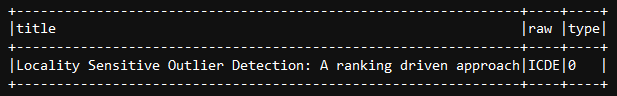
\includegraphics[width=1\textwidth]{query/spark_q1.PNG}
\label{fig:query1}
\end{figure}

\subsection{Query 2 - WHERE, LIMIT, LIKE}
This query returns the articles whose title string contains \emph{"Machine Learning"}.\newline
\textbf{Description:} we filter the articles whose title contains "Machine Learning" using the like operator. Results are then limited
to 3 tuples and projected over the article title.\newline
\begin{python}
df_articles.filter(f.col("title").like("%Machine Learning%"))\
           .limit(3)\
           .select("title")\
           .show(truncate=False)
\end{python}
\begin{figure}[H]
\centering
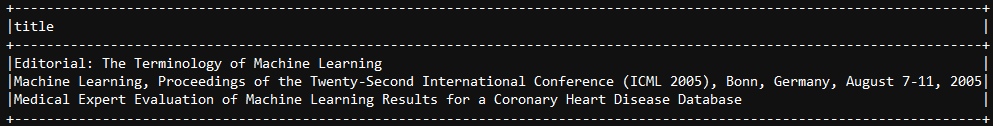
\includegraphics[width=1\textwidth]{query/spark_q2.PNG}
\label{fig:query2}
\end{figure}

\subsection{Query 3 - WHERE, IN, NESTED QUERY}
This query finds authors that has the same nationality of at least one of the authors of \emph{"Locality Sensitive Outlier
Detection: A ranking driven approach"} article.\newline
\textbf{Description:} this query has been splitted in 2 queries:
                        \begin{itemize}
                            \item \emph{First query:} articles are filtered to find the article with the given title. After that,
                                the authors array is exploded to perform a join on its idAuth field with the authors dataframe.
                                Finally, nationalities of the article's authors are collected into a list using the \verb |collect_set|.\newline
                                \verb|collect_set|, as the name suggests, discards duplicates, so the final list is a set of nationalities.
                            \item \emph{Second query:} starting from the authors' dataframe, we filtered all the authors whose nationality is
                                present inside the list created with the previous query.\\
                        \end{itemize}
\begin{python}
nationalities_list = df_articles.filter(f.col("title") == "Locality Sensitive Outlier Detection: A ranking driven approach")\
                                .select(f.explode(df_articles.authors.idAuth).alias("idAuth"))\
                                .join(df_authors, on=f.col("idAuth") == df_authors._id)\
                                .select("nationality")\
                                .agg(f.collect_set("nationality")).collect()[0][0]

df_authors.filter(f.col("nationality")\
          .isin(nationalities_list))\
          .select("name","nationality")\
          .show(truncate=False)
\end{python}
\begin{figure}[H]
\centering
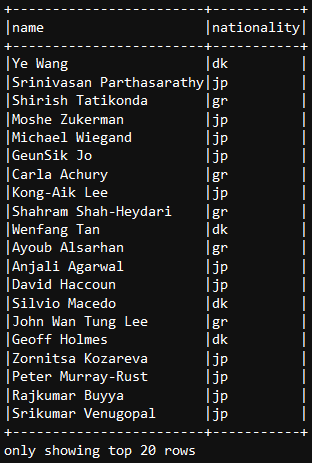
\includegraphics[width=0.4\textwidth]{query/spark_q3.PNG}
\label{fig:query3}
\end{figure}

\subsection{Query 4 - GROUP BY, JOIN, AS}
This query finds the 3 most frequent keywords of articles written by italian authors.\newline
\textbf{Description:} starting from the authors dataframe, we keep only italian authors and explode the articles field, renaming the
new obtained field to \verb |articles|. After that, duplicates are discarded.\newline
In the second part of the query, we load the full articles's rows using a join. Then, keywords array is exploded. Keywords are grouped
and counted. The groups are finally sorted and limited to show the top 3 keywords.\newline
\begin{python}
df_italian = df_authors.filter(f.col("nationality") == "it")\
                       .select(f.explode("articles")).withColumnRenamed("col","articles")\
                       .distinct()

df_keywords = df_italian.join(df_articles, df_italian.articles == df_articles._id, "inner")\
                        .select("articles", f.explode("keywords")).withColumnRenamed("col","keywords")\
                        .groupby("keywords")\
                        .agg(f.count("keywords").alias("n_occurences"))\
                        .sort("n_occurences", ascending=False)\
                        .limit(3).show()
\end{python}
\begin{figure}[H]
\centering
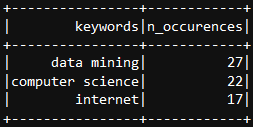
\includegraphics[width=0.3\textwidth]{query/spark_q4.PNG}
\label{fig:query4}
\end{figure}

\subsection{Query 5 - WHERE, GROUP BY}
This query finds the cities with more than 65 venues.\newline
\textbf{Description:} the venues dataframe is grouped with respect to the city to perform the count. After that, we keep only cities with
more than 65 venues and sort the result in descending order.\newline
\begin{python}
df_venues\
    .groupby("city")\
    .count()\
    .filter(f.col("count") > 65)\
    .sort("count", ascending=False).show()
\end{python}
\begin{figure}[H]
\centering
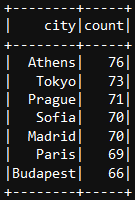
\includegraphics[width=0.2\textwidth]{query/spark_q5.PNG}
\label{fig:query5}
\end{figure}

\subsection{Query 6 - GROUP BY, HAVING, AS}
This query finds the field of studies that appears more than 15 times.\newline
\textbf{Description:} We use the explode function to convert the fos array into multiple rows,then we rename the resulting column to
\verb |fos|, group by \verb|fos| and count the number of occurrences.\newline
After that, we keep rows with more than 15 occurrences, sort the remaining rows in descending order based on the number of occurrences,
and show the top rows.\newline
\begin{python}
df_articles\
    .select("_id", "title", f.explode("fos")).withColumnRenamed("col", "fos")\
    .groupby("fos")\
    .agg(f.count("fos").alias("n_occurencies"))\
    .filter(f.col("n_occurencies") > 15)\
    .sort("n_occurencies", ascending=False)\
    .show(truncate=False)
\end{python}
\begin{figure}[H]
\centering
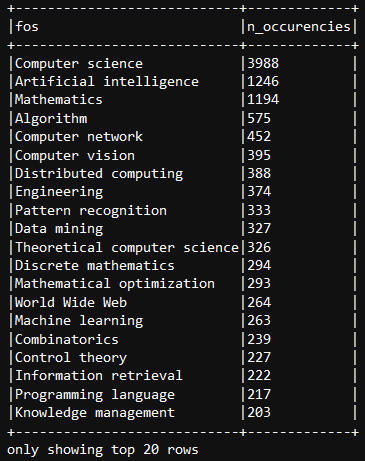
\includegraphics[width=0.5\textwidth]{query/spark_q6.PNG}
\label{fig:query6}
\end{figure}

\subsection{Query 7 - WHERE, GROUP BY, HAVING, AS}
This query finds all the volumes with at least 5 articles in the dataset, published after 2000.\newline
\textbf{Description:} This query filters the articles in the articles dataframe to only those published after the year 2000,
then groups the remaining articles by \verb|venue_raw| and \verb|volume|, counts the number of articles per group, filters the
groups to only those with more than 4 articles, and finally displays the results.\newline
\begin{python}
df_articles\
    .filter(f.col("year") > 2000)\
    .groupby("venue_raw", "volume")\
    .agg(f.count("volume").alias("num_articles"))\
    .filter(f.col("num_articles") > 4)\
    .show(truncate = False)
\end{python}
\begin{figure}[H]
\centering
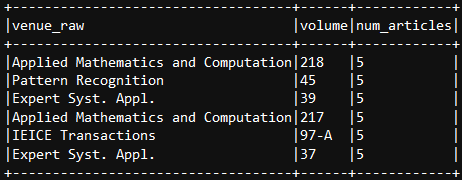
\includegraphics[width=0.8\textwidth]{query/spark_q7.PNG}
\label{fig:query7}
\end{figure}

\subsection{Query 8 - WHERE, NESTED QUERY, GROUP BY}
The following query is divided in two queries:
\begin{itemize}
    \item[\textbf{8a.}] find the venue with highest number of articles
    \item[\textbf{8b.}] find the number of articles published per year on that venue
\end{itemize}
\textbf{Description:} the basic functionalities of the two queries are the following
                    \begin{itemize}
                        \item the \emph{first query} selects the top venue from the venue dataframe based on the size of the \verb|artIds| attribute
                        \item the \emph{second query} filters articles with the selected \verb|venue_raw|, groups the articles by year, and counts the number
                            of articles in each group. Finally, it displays the results projecting over \verb|top_venue|, \verb|year| and \verb|articles_count| \\
                    \end{itemize}
\begin{python}
top_venue = df_venues\
                .select("raw",f.size("artIds").alias("count"))\
                .orderBy("count",ascending = False)\
                .limit(1)

df_articles_year = df_articles\
                        .filter(f.col("venue_raw") == top_venue.collect()[0][0])\
                        .groupBy("year")\
                        .count()\
                        .orderBy("count",ascending=False)\
                        .select(f.lit(top_venue.collect()[0][0]).alias("VenueRAW"),"year",f.col("count").alias("articles_count"))\
                        .show(truncate=False)
\end{python}
\begin{figure}[H]
\centering
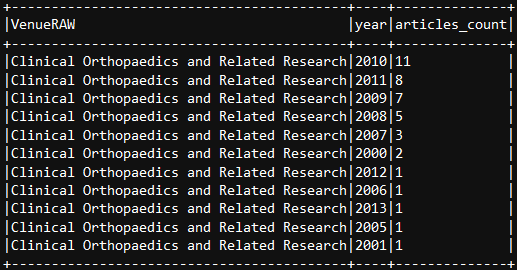
\includegraphics[width=0.8\textwidth]{query/spark_q8.PNG}
\label{fig:query8}
\end{figure}

\subsection{Query 9 - WHERE, GROUP BY, HAVING, 1 JOIN}
The following query finds the articles, published after 2000, with more than 13 different nationalities of its authors.\newline
\textbf{Description:} this query filters the articles dataframe by year, exploding the authors array \verb|idAuth| field (note that
authors is an array of struct elements with 2 fields). After that, it joins the result with the authors dataframe, groups the
articles by id and counts the number of distinct nationalities among the authors. It finally filters the results to include only
articles with more than 13 different nationalities and orders the results in descending order, displaying the title of the article,
the list of nationalities and their count.\newline
\begin{python}
df_articles_nationalities = df_articles.alias("art")\
                                .filter(f.col("year") > 2000)\
                                .select("art._id","art.title", f.explode("art.authors.idAuth").alias("author"))\
                                .join(df_authors.alias("auth"), on=f.col("author") == df_authors._id)\
                                .groupBy("art._id")\
                                .agg(f.first("title").alias("title"),f.countDistinct("nationality").alias("different_nationalities"), f.collect_set("nationality").alias("nationalities_list"))\
                                .filter(f.col("different_nationalities") > 13)\
                                .orderBy("different_nationalities",ascending=False)\
                                .select("title","different_nationalities",f.sort_array("nationalities_list").alias("nationalities_list"))\
                                .show(truncate=False)
\end{python}
\begin{figure}[H]
\centering
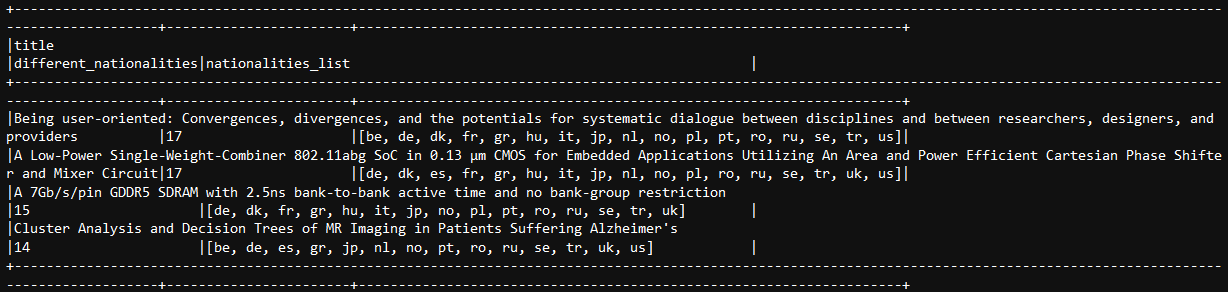
\includegraphics[width=1\textwidth]{query/spark_q9.PNG}
\label{fig:query9}
\end{figure}

\subsection{Query 10 - WHERE, GROUP BY, HAVING, 2 JOINS}
This query finds  all the authors that published on more than 2 Journals.\newline
\textbf{Description:}  starting from the authors dataframe, we explode the articles array, creating a new field named \verb|article|.
After that, we join the results with the articles collection and then with the venues collection. Then, we filter the results to keep
only articles written on journals (type 1) and group by the author id. Finally, we count the number of distinct venues in each group
(collecting in a list all the venues of the group), and keep only the groups with more than 2 venues.
\begin{python}
df_exploded_authors = df_authors.alias("auth")\
                        .select("auth._id","auth.name", f.explode("auth.articles").alias("article"))\
                        .join(df_articles.alias("art"), on=f.col("article") == df_articles._id)\
                        .select("auth._id","auth.name","art._id","art.venue_raw")\
                        .join(df_venues.alias("ven"), on=f.col("venue_raw") == df_venues.raw)\
                        .filter(f.col("type") == 1)\
                        .groupBy("auth._id")\
                        .agg(f.first("name").alias("name"),f.countDistinct("raw").alias("venue_count"),f.concat_ws(" - ",f.collect_set("raw")).alias("venues_list"))\
                        .filter(f.col("venue_count") > 2)\
                        .orderBy("venue_count", ascending=False).show(3,truncate=False)
\end{python}
\begin{figure}[H]
\centering
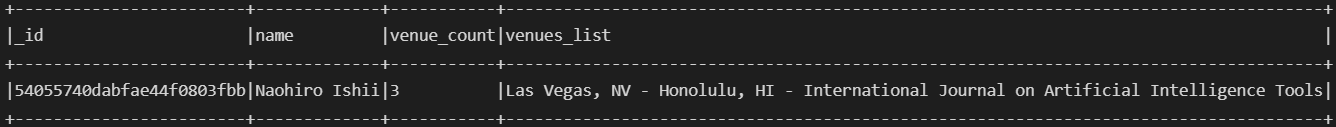
\includegraphics[width=1\textwidth]{query/spark_q10.PNG}
\label{fig:query10}
\end{figure}

\subsection{Query 11 - EXTRA}
This query returns all the articles written by authors whose names combined have all 26 letters of the alphabet.\newline
\textbf{Description:} The query starts with exploding articles for each author. Then, the grouping combined with the collect
retrieves, for each article, the list of its authors, then several operation are applied on this list in order to obtain the
different letters that are present in the list of authors. After that, a filter to keep only the ones that have all the 26
letters of the alphabet in it is applied, and the result is joined with articles to obtain the title. Finally, a projection is
used to display the title and the list of authors in alphabetical order.\newline
\begin{python}
df_authors.select("name", f.explode("articles").alias("idArt")) \
          .groupBy("idArt") \
          .agg(f.collect_set("name").alias("authorsList")) \
          .select("idArt", "authorsList", (f.size(f.array_distinct(f.split(f.regexp_replace(f.lower(f.concat_ws("", "authorsList")), "[^a-z]", ""), "")))-1).alias("differentLetters")) \
          .filter(f.col("differentLetters") == 26)\
          .join(df_articles, on=f.col("idArt") == df_articles._id) \
          .select("title", f.concat_ws(", ", f.sort_array("authorsList")).alias("authorsList"), "differentLetters") \
          .show(truncate=False)
\end{python}
\begin{figure}[H]
\centering
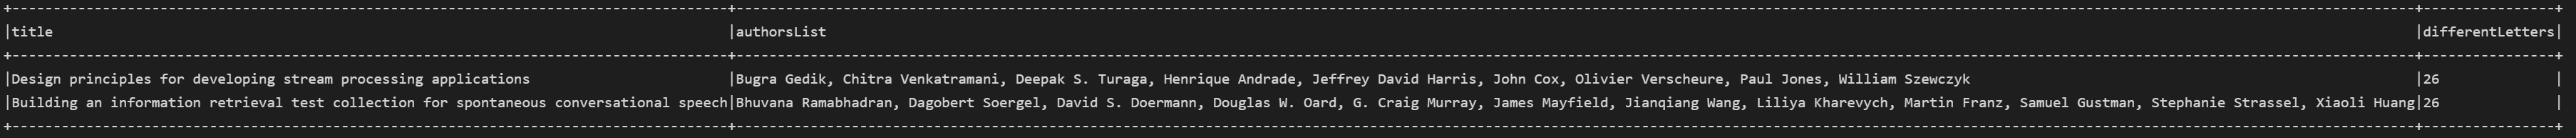
\includegraphics[width=1\textwidth]{query/spark_q11.PNG}
\label{fig:query11}
\end{figure}

\subsection{Query 12 - EXTRA}
This query returns all articles written in affiliation with \emph{Politecnico of Milano}.\newline
\textbf{Description:} the query starts by exploding the authors array field in the article, creating the new \verb|affiliation| attribute.
Articles that contain at least one of the desired organization (the same article could be written in collaboration with different
universities) are kept. Then, a join with the authors collection is executed to retrieve the name of the author.
\begin{python}
df_articles\
    .select("title",f.explode("authors").alias("affiliation"))\
    .filter(f.col("affiliation.org").like("%Poli%Mil%"))\
    .join(df_authors, on=f.col("affiliation.idAuth") == df_authors._id) \
    .select("title", "name", "affiliation.org") \
    .orderBy("title","name")\
    .show(truncate=False)
\end{python}
\begin{figure}[H]
\centering
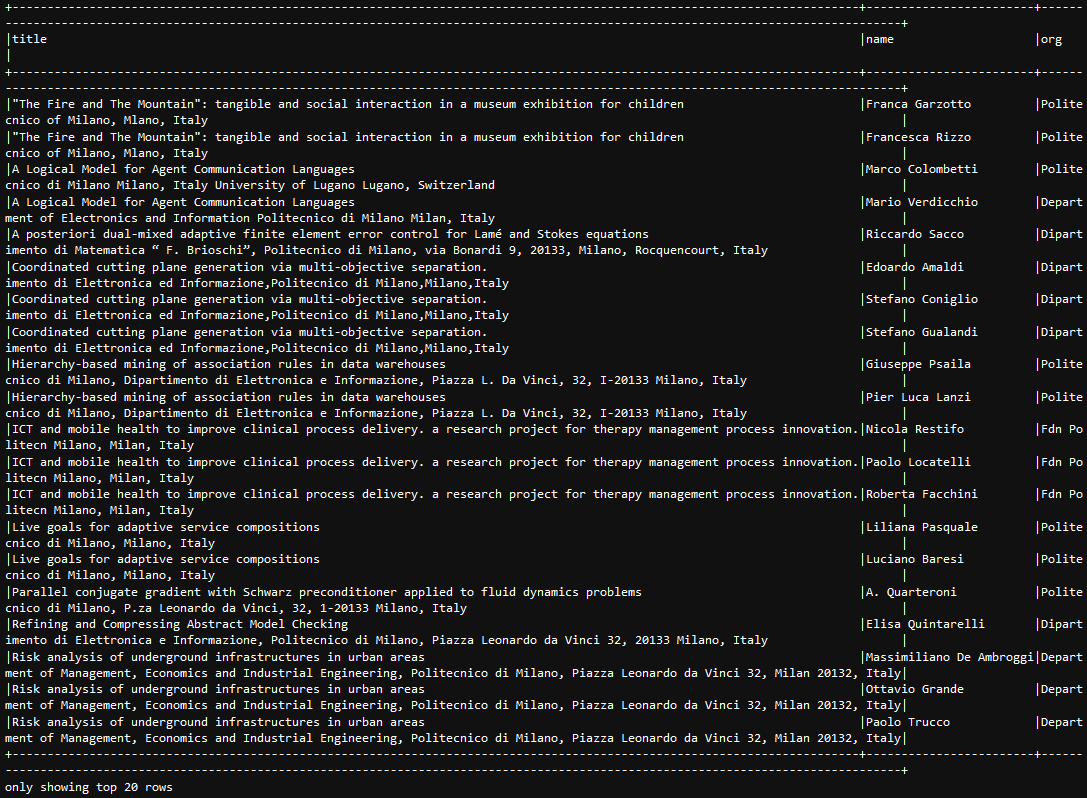
\includegraphics[width=1\textwidth]{query/spark_q12.PNG}
\label{fig:query12}
\end{figure}


\chapter{Conclusions}
\label{ch:conclusions}
Spark is a computing platform designed to efficiently scale data processing and analysis.
Indeed, given its distributed framework and the use of RDDs, it allows splitting the workload across multiple nodes.
Furthermore, Spark offers a rich set of APIs and libraries, making it a versatile tool for working with big data.
In our implementation, we used the PySpark interface, which makes the interaction with Apache very intuitive.
The flexibility offered by the RDDs made it possible to shape the data structure to match our needs.

In the end, the technologies used in the project, allowed us to face, from different perspectives, the challenges of
designing efficient database solutions for large sets of data.


\end{document}
